\chapter{Взаимодействие волноводов}
\section{Поле цилиндрического волноовда}
Поле в волноводе в некотором приближении - это распределение Гаусса. Также для упрощения, пользуясь симметрией цилиндрического волновода сначала рассмотрим двухмерный случай, зависимость только от одной координаты:
\begin{equation}
  \label{gauss}
  E(x)=\frac{1}{\sigma\sqrt{2\pi}}\exp\left(-\frac{x^2}{2\sigma^2}\right)
\end{equation}
Таким образом мы получим нормальное распределение с вершиной в точке $(0,0)$.
Здесь $\sigma = 1,1a$ - параметр распределения, равен 1,1 радиуса волновода
Для сравнения, на рисунке \ref{diameter} показаны распределния поля волноводов разной толщины

\begin{figure}[h!]
	\begin{minipage}[h]{0.49\linewidth}
		\center{\includegraphics[width=1\linewidth]{img/field_distribution.png} \\ а)}
	\end{minipage}
	\hfill
	\begin{minipage}[h]{0.49\linewidth}
		\center{\includegraphics[width=1\linewidth]{img/field_distribution2.png} \\ б)}
	\end{minipage}
	\caption{Распределение поля в волноводах с разным радиусом моды: \mbox{а) 7~мкм, б) 4~мкм}}
	\label{diameter}
\end{figure}

Целью данной работы является рассмотрение эффективности передачи энергии при соединении волноводов. Опишем эту зависимость теоретически.

Из Лефевра известно, что отношение интенсивности $C$ это отношение скалярного квадрата мощности связанной волны к скалярному квадрату мощности входной волны. Его можно найти по формуле:

\begin{equation}
	\label{coupling_full}
	C = \frac{\left[\int\limits_{-\infty}^{\infty}E_{in}(x)e_{f0}^*(x) \,dx\right]^2}
	{\int\limits_{-\infty}^{\infty}e_{f0}(x)e_{f0}^*(x) \,dx
	 \int\limits_{-\infty}^{\infty}E_{in}(x)E_{in}^*(x) \,dx}
\end{equation}

Так как мы рассматриваем только действительную часть распределения, то формула упрощается:

\begin{equation}
	\label{coupling}
	C = \frac{\left[\int\limits_{-\infty}^{\infty}E_{in}(x)e_{f0}(x) \,dx\right]^2}
	{\int\limits_{-\infty}^{\infty}e_{f0}(x)^2 \,dx
	 \int\limits_{-\infty}^{\infty}E_{in}(x)^2 \,dx}
\end{equation}

Это выражение называется интегралом перекрытия  и показывает, какая часть энергии перейдет в возбуждение моды во втором волноводе. 

\begin{figure}[h!]
	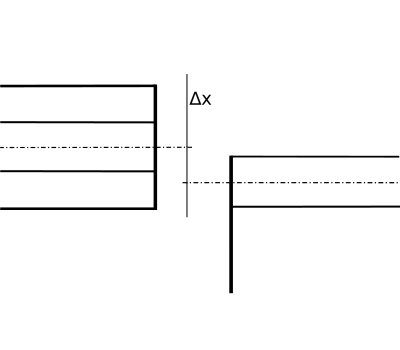
\includegraphics[width=.5\textwidth]{img/transverse_movement.pdf}
	\caption{Поперечное смещение волноводов}
\end{figure}

В зависимости от взаимного расположения волноводов изменяется расположение распределений под интегралом и соответственно изменяется итоговое значение.

В случае поперечного смещения, взаимное положение полей мод принимает такой вид:

\begin{figure}[h!]
	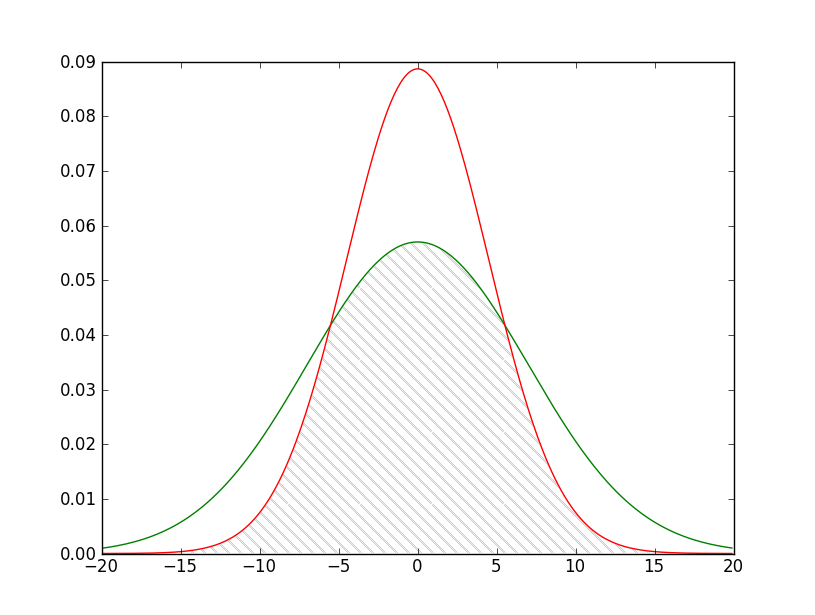
\includegraphics[width=.5\textwidth]{img/intersection.png}
	\caption{Распределение полей при поперечнои смещении}
\end{figure}

Поле возбуждаемой моды имеет максимум при $x=0$, а поле в входном волноводе имеет максимум в точке $x=4$. Это несоответствие уменьшает выходную мощность моды. Очевидно что коэффициент передачи максимален и равен 1 при условии $E_{in} = e_{f0}$ для всех $x$

\section{Поле волноводов в пространстве}

Выше рассматривался двухмерный случай распределения поля. В трехмерном случае нормальное распределение зависит от двух координат и равно:
\begin{equation}
  \label{gauss3d}
  E(x,y)=\frac{1}{2\pi\sigma_1\sigma_2}\exp\left(-\frac{x^2}{2\sigma_1^2}-\frac{y^2}{2\sigma_2^2}\right)
\end{equation}
где $\sigma_1$ и $\sigma_2$ - радиус моды по осям $x$ и $y$ соответственно. График этого уравнения выглядит представлен на рисунке \ref{gauss3dPlot}.

Аналогично двухмерному случаю, найдем интеграл перекрытия.

\begin{equation}
	\label{coupling}
	C = \frac{\left[\iint\limits_{-\infty}^{\infty}E_{in}(x,y)e_{f0}(x,y) \,dxdy\right]^2}
	{\iint\limits_{-\infty}^{\infty}e_{f0}(x,y)^2 \,dxdy
	 \iint\limits_{-\infty}^{\infty}E_{in}(x,y)^2 \,dxdy}
\end{equation}

\begin{figure}[h!]
	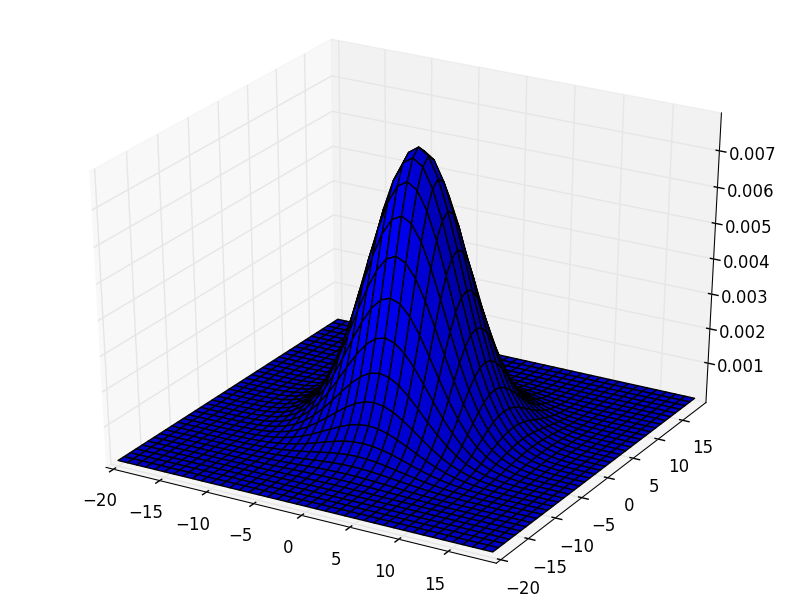
\includegraphics[width=0.5\textwidth]{img/gauss3d.png}
	\caption{Распределение Гаусса в пространстве}
	\label{gauss3dPlot}
\end{figure}

